\documentclass[10pt,a4paper,onecolumn]{article}
% \usepackage[utf8]{inputenc}
\usepackage{marginnote}
\usepackage{graphicx}
\usepackage{xcolor}
\usepackage{authblk,etoolbox}
\usepackage{titlesec}
\usepackage{calc}
\usepackage{hyperref}
\hypersetup{breaklinks=true,
            bookmarks=true,
            pdfauthor=
{
      Florian Muellerklein,
  },
            pdftitle=
{
[Re] Reproducing CIFAR-10 results from deep and wide preactivation residual
networks
},
            colorlinks=true,
            citecolor=blue,
            urlcolor=blue,
            linkcolor=blue,
            pdfborder={0 0 0}}
\urlstyle{same}
\usepackage{tcolorbox}
\usepackage{ragged2e}
\usepackage{fontspec}
\usepackage{fontawesome}
\usepackage{caption}
\usepackage{listings}
\lstnewenvironment{code}{\lstset{language=Haskell,basicstyle=\small\ttfamily}}{}



%\usepackage{fancyvrb}
%\VerbatimFootnotes
%\usepackage{graphicx}
%\usepackage{mdframed}
%\newmdenv[backgroundcolor=lightgray]{Shaded}


\usepackage{longtable,booktabs}

\usepackage[
  backend=biber,
%  style=alphabetic,
%  citestyle=numeric
]{biblatex}
\bibliography{pre_and_wide_resnets.bib}



% --- Macros ------------------------------------------------------------------
\renewcommand*{\bibfont}{\small \sffamily}

\definecolor{red}{HTML}{CF232B}
\newcommand{\ReScience}{Re{\bfseries \textcolor{red}{Science}}}

\newtcolorbox{rebox}
   {colback=blue!5!white, colframe=blue!40!white,
     boxrule=0.5pt, arc=2pt, fonttitle=\sffamily\scshape\bfseries,
     left=6pt, right=20pt, top=6pt, bottom=6pt}

\newtcolorbox{repobox}
   {colback=red, colframe=red!75!black,
     boxrule=0.5pt, arc=2pt, left=6pt, right=6pt, top=3pt, bottom=3pt}

% fix for pandoc 1.14     
\newcommand{\tightlist}{%
  \setlength{\itemsep}{1pt}\setlength{\parskip}{0pt}\setlength{\parsep}{0pt}}

% --- Style -------------------------------------------------------------------
\renewcommand*{\bibfont}{\small \sffamily}
\renewcommand{\captionfont}{\small\sffamily}
\renewcommand{\captionlabelfont}{\bfseries}

\makeatletter
\renewcommand\@biblabel[1]{{\bf #1.}}
\makeatother

% --- Page layout -------------------------------------------------------------
\usepackage[top=3.5cm, bottom=3cm, right=1.5cm, left=1.5cm,
            headheight=2.2cm, reversemp, includemp, marginparwidth=4.5cm]{geometry}

% --- Section/SubSection/SubSubSection ----------------------------------------
\titleformat{\section}
  {\normalfont\sffamily\Large\bfseries}
  {}{0pt}{}
\titleformat{\subsection}
  {\normalfont\sffamily\large\bfseries}
  {}{0pt}{}
\titleformat{\subsubsection}
  {\normalfont\sffamily\bfseries}
  {}{0pt}{}
\titleformat*{\paragraph}
  {\sffamily\normalsize}


% --- Header / Footer ---------------------------------------------------------
\usepackage{fancyhdr}
\pagestyle{fancy}
%\renewcommand{\headrulewidth}{0.50pt}
\renewcommand{\headrulewidth}{0pt}
\fancyhead[L]{\hspace{-1cm}
\includegraphics[width=4.0cm]{rescience-logo.pdf}}
\fancyhead[C]{}
\fancyhead[R]{} 
\renewcommand{\footrulewidth}{0.25pt}

\fancyfoot[L]{\hypersetup{urlcolor=red}
              \sffamily \ReScience~$\vert$
              \href{http://rescience.github.io}{rescience.github.io}
              \hypersetup{urlcolor=blue}}
\fancyfoot[C]{\sffamily \thepage}
\fancyfoot[R]{\sffamily Sep 2015 $\vert$
                        Volume \textbf{1} $\vert$
                        Issue \textbf{1}}
\pagestyle{fancy}
\makeatletter
\let\ps@plain\ps@fancy
\fancyheadoffset[L]{4.5cm}
\fancyfootoffset[L]{4.5cm}

% --- Title / Authors ---------------------------------------------------------
% patch \maketitle so that it doesn't center
\patchcmd{\@maketitle}{center}{flushleft}{}{}
\patchcmd{\@maketitle}{center}{flushleft}{}{}
% patch \maketitle so that the font size for the title is normal
\patchcmd{\@maketitle}{\LARGE}{\LARGE\sffamily}{}{}
% patch the patch by authblk so that the author block is flush left
\def\maketitle{{%
  \renewenvironment{tabular}[2][]
    {\begin{flushleft}}
    {\end{flushleft}}
  \AB@maketitle}}
\makeatletter
\renewcommand\AB@affilsepx{ \protect\Affilfont}
%\renewcommand\AB@affilnote[1]{{\bfseries #1}\hspace{2pt}}
\renewcommand\AB@affilnote[1]{{\bfseries #1}\hspace{3pt}}
\makeatother
\renewcommand\Authfont{\sffamily\bfseries}
\renewcommand\Affilfont{\sffamily\small\mdseries}
\setlength{\affilsep}{1em}

\LetLtxMacro{\OldIncludegraphics}{\includegraphics}
\renewcommand{\includegraphics}[2][]{\OldIncludegraphics[width=12cm, #1]{#2}}


% --- Document ----------------------------------------------------------------
\title{[Re] Reproducing CIFAR-10 results from deep and wide preactivation residual
networks}

    \usepackage{authblk}
                        \author[1]{Florian Muellerklein}
                            \affil[1]{}
            
\date{\vspace{-5mm}
      \sffamily \small \href{mailto:f.muellerklein@gmail.com}{f.muellerklein@gmail.com}}


\setlength\LTleft{0pt}
\setlength\LTright{0pt}


\begin{document}
\maketitle

\marginpar{
  %\hrule
  \sffamily\small
  %\vspace{2mm}
  {\bfseries Editor}\\
  Name Surname\\

  {\bfseries Reviewers}\\
        Name Surname\\
        Name Surname\\
  
  {\bfseries Received}  Sep, 1, 2015\\
  {\bfseries Accepted}  Sep, 1, 2015\\
  {\bfseries Published} Sep, 1, 2015\\

  {\bfseries Licence}   \href{http://creativecommons.org/licenses/by/4.0/}{CC-BY}

  \begin{flushleft}
  {\bfseries Competing Interests:}\\
  The authors have declared that no competing interests exist.
  \end{flushleft}

  \hrule
  \vspace{3mm}

  \hypersetup{urlcolor=white}
  
    \vspace{-1mm}
  \begin{repobox}
    \bfseries\normalsize
      \href{https://github.com/FlorianMuellerklein/ReScience-submission/tree/master/article}{\faGithubAlt~Article repository}
  \end{repobox}
      \vspace{-1mm}
  \begin{repobox}
    \bfseries\normalsize
      \href{https://github.com/FlorianMuellerklein/ReScience-submission/tree/master/code}{\faGithubAlt~Code repository}
  \end{repobox}
      \vspace{-1mm}
  \begin{repobox}
    \bfseries\normalsize
      \href{https://github.com/FlorianMuellerklein/ReScience-submission/tree/master/data}{\faGithubAlt~Data repository}
  \end{repobox}
      \hypersetup{urlcolor=blue}
}

\begin{rebox}
\sffamily {\bfseries A reference implementation of}
\small
\begin{flushleft}
\begin{itemize}
    \item[→] Original article (Identity Mappings in Deep Residual Networks, Kaiming
He, Xiangyu Zhang, Shaoqing Ren, and Jian Sun, arXiv preprint
arXiv:1603.05027, 12, April 2016)
  \end{itemize}\par
\end{flushleft}
\end{rebox}


\section{Introduction}\label{introduction}

In 2015, Deep Residual Networks {[}1{]} were introduced as the winning
solutions to ImageNet detection, ImageNet localization, COCO detection,
and COCO segmentation, and they made it possible to train extremely deep
neural networks of up to 1000 or more layers. The main idea is that
Residual Networks ``reformulate the layers as learning residual
functions with reference to the layer inputs, instead of learning
unreferenced functions'' {[}1{]}. The basic idea is that the residual
functions (blocks) are a combination of convolution layers and skip
connections. The residual blocks are basically two branches that come
together with an element-wise addition. One branch of the residual block
is a stack of two convolution layers and the other is an identity
function.

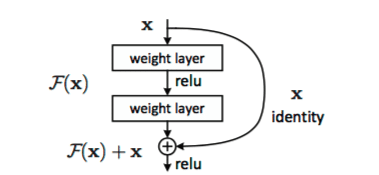
\includegraphics{images/residual_block.png}

Diagram of the residual block taken from {[}1{]}.

Just like with normal convolution layers, these residual blocks can be
layered to create networks of increasing depth. Below is the basic
structure of the CIFAR-10 residual network {[}1{]}{[}2{]}, with the
depth being controlled by a multiplier \emph{n} which dictates how many
residual blocks to insert between each downsampling layer. Downsampling
is done by increasing the stride of the first convolution layer in a
residual block. Whenever the number of filters are increased the first
convolution layer within a residual block will do the downsampling.

\begin{longtable}[c]{@{}lcc@{}}
\toprule
Group & Size & Multiplier\tabularnewline
\midrule
\endhead
Conv1 & {[}3x3, 16{]} & -\tabularnewline
Conv2 & {[}3x3, 16{]}{[}3x3, 16{]} & \emph{n}\tabularnewline
Conv3 & {[}3x3, 32{]}{[}3x3, 32{]} & \emph{n}\tabularnewline
Conv4 & {[}3x3, 64{]}{[}3x3, 64{]} & \emph{n}\tabularnewline
Avg-Pool & 8x8 & -\tabularnewline
Softmax & 10 & -\tabularnewline
\bottomrule
\end{longtable}

Basic structure of the CIFAR-10 Residual Network. An initial convolution
layer is followed by residual blocks of two 3x3 convolutions which are
parallel to identity mappings, the output of the identity and
convolution stacks are added after each block. The depth is mostly
altered by the multiplier n which defines how many residual blocks to
use in each section.

In addition to the stacked 3x3 convolution architecture, ``Deep Residual
Learning for Image Recognition'' also introduces a bottleneck
architecture which is designed to increase the depth without
significantly increasing the amount of parameters.{[}1{]} The structure
of this architecture can be seen below, the depth is still controlled by
a multiplier \emph{n}. The main changes are in the residual blocks.

\begin{longtable}[c]{@{}lcc@{}}
\toprule
Group & Size & Multiplier\tabularnewline
\midrule
\endhead
Conv1 & {[}3x3, 16{]} & -\tabularnewline
Conv2 & {[}1x1, 16{]}{[}3x3, 16{]}{[}1x1, 64{]} &
\emph{n}\tabularnewline
Conv3 & {[}1x1, 32{]}{[}3x3, 32{]}{[}1x1, 128{]} &
\emph{n}\tabularnewline
Conv4 & {[}1x1, 64{]}{[}3x3, 64{]}{[}1x1, 256{]} &
\emph{n}\tabularnewline
Avg-Pool & 8x8 & -\tabularnewline
Softmax & 10 & -\tabularnewline
\bottomrule
\end{longtable}

This reproduction will focus on two recent improvements on the original
residual network design, Preactivation Residual Networks and Wide
Residual Networks.{[}2{]}{[}3{]} The preactivation architecture switches
up the order of the convolution, batch normalization and nonlinearities
within each residual block. The wide architecture simply increases the
number of convolution kernels within each preactivation residual block.

\textbf{Preactivation Residual Blocks:} ``Identity Mappings in Deep
Residual Networks'' {[}2{]} introduces the preactivation architecture
which changes the order of the convolution kernels, batch
normalizations, and nonlinearities. The preactivation residual block is
said to be easier to optimize and has implicit regularization.{[}2{]}
The changes from the original residual block to the preactivation
residual block are best viewed in the figure below.

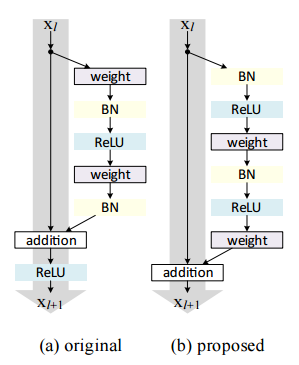
\includegraphics{images/pre_block.png}

The alterations from the original ResNet to the Preactivation ResNet.

\textbf{Wide Residual Networks:} The preactivation residual networks are
very deep but also very thin, so ``Wide Residual Networks'' {[}3{]}
suggested that better improvements can be realized with a much more
shallow and wide architecture. With normal residual networks we get
diminishing returns in performance by increasing the depth. The wide
residual networks are an attempt to mitigate this observation. The
authors introduce ``wider deep residual networks that significantly
improve over {[}2{]}, having 50 times less layers and being more than 2
times faster.'' {[}3{]} Their 16-layer wide residual Network performs as
well as a thin 1001-layer preactivation residual network. The authors
also claim that the wider networks are much more efficient on a GPU than
the deeper thin networks.{[}3{]}

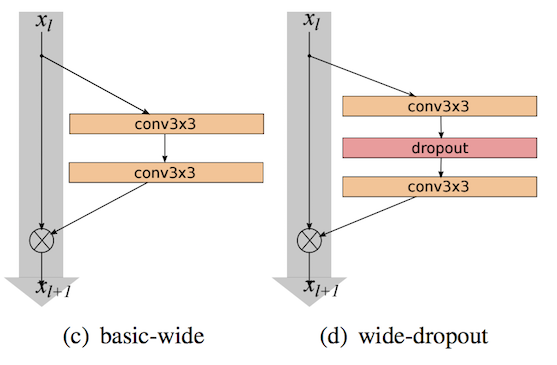
\includegraphics{images/wide_block.png}

An example of the wide ResNet, it's basically a Preactivation ResNet
with an increased filter count in the residual blocks and an optional
dropout between the two convolution layers.

The wide-ResNet simply adds another multiplier \emph{k} that increases
the number of filters used in each residual block. The idea of adding
dropout in between the two convolution layers is also introduced with
the wider residual blocks. The basic structure can be seen below.

\begin{longtable}[c]{@{}lcc@{}}
\toprule
Group & Size & Multiplier\tabularnewline
\midrule
\endhead
Conv1 & {[}3x3, 16{]} & -\tabularnewline
Conv2 & {[}3x3, 16 x \emph{k}{]}{[}3x3, 16 x \emph{k}{]} &
\emph{n}\tabularnewline
Conv3 & {[}3x3, 32 x \emph{k}{]}{[}3x3, 32 x \emph{k}{]} &
\emph{n}\tabularnewline
Conv4 & {[}3x3, 64 x \emph{k}{]}{[}3x3, 64 x \emph{k}{]} &
\emph{n}\tabularnewline
Avg-Pool & 8x8 & -\tabularnewline
Softmax & 10 & -\tabularnewline
\bottomrule
\end{longtable}

\section{Methods}\label{methods}

Both the original residual network and follow up preactivation residual
network papers use identical preprocessing, training and regularization
parameters. However, the wide residual paper uses different
preprocessing, training, and regularization while still comparing
results to the previous preactivation residual network. For wide
residual networks they used ``global contrast normalization and ZCA
whitening''{[}3{]} to preprocess the CIFAR-10 images. However, the
Microsoft Research Asia group only used ``32×32 images, with the
per-pixel mean subtracted''{[}1{]} as their network inputs. It is
possible that different network architectures would require different
parameters and input data to achieve their best performance. But there
should also be comparisons done where everything stays exactly the same
except for the networks. This reproduction will be done using the
preprocessing, training and regularization parameters from the original
and preactivation residual network papers.{[}1{]}{[}2{]}

\textbf{Preprocessing:} The only preprocessing done to the CIFAR-10
images are per-pixel mean subtraction as in {[}1{]} and {[}2{]}.

\textbf{Data Augmentation:} As the data were fed into the network they
were zero-padded with 4 pixels on every side and a random crop was taken
of the original size of 32x32. This effectively results in random
translations. Additionally, a horizontal flip was applied with
probability 0.5. Unfortunately batch sizes of 128 could not be used and
instead batch sizes of 64 had to be used due to hardware constraints.

\textbf{Training and regularization:} The networks were trained with 200
epochs (full passes through training dataset) with stochastic gradient
descent, nesterov momentum of 0.9, and cross-entropy loss. For the
bottleneck architecture, the initial learning rate was set to 0.01 to
warm up the network and was increased to 0.1 at epoch 10 then continued
on the same schedule as the other networks. For all other networks the
learning rate was adjusted by the following schedule \{0:0.1, 80: 0.01,
120: 0.001\}. L2 regularization of 0.0001 was used used as in
{[}1{]}{[}2{]} and not 0.0005 like in {[}3{]}.

\textbf{Dropout:} Dropout of 0.3 was used in the wide residual
network.{[}3{]}

\textbf{Hardware and software:} This reproduction was done using the
Theano and Lasagne software frameworks for mathematical computation and
neural networks.{[}4{]}{[}5{]} A Nvidia GTX 980 GPU was used to train
and evaluate the networks. Although the impact should be insignificant
it is worth noting that the original papers were both done with the
Torch software package and a GPU with the same underlying architecture
but more memory.{[}6{]}

\section{Results}\label{results}

The reproduction results are consistent with those of the original paper
within a reasonable margin. The training parameters and preprocessing
were kept the same to the extent possible. The most notable exceptions
are the batchsize (due to hardware constraints) and the training
parameters for the wide residual network.

\begin{longtable}[c]{@{}ccc@{}}
\toprule
\textbf{ResNet Type} & \textbf{Original Paper} & \textbf{Test
Results}\tabularnewline
\midrule
\endhead
ResNet-110 & 6.37 & 6.38\tabularnewline
ResNet-164 & 5.46 & 5.66\tabularnewline
WResNet-n2-k4 & 5.55 & 5.41\tabularnewline
\bottomrule
\end{longtable}

All results are presented from the first and only training run. I did
not run each network multiple times and choose the best score.

Additionally, the training plots seemed to have the same characteristics
as those presented in the original papers. Training plots for residual
networks are characterized by fairly noisy trends in the cross-entropy
during training and also much less of a quadratic trend than seen in
other neural networks. These trends are also seen here.

\subsubsection{ResNet-110}\label{resnet-110}

\begin{figure}[htbp]
\centering
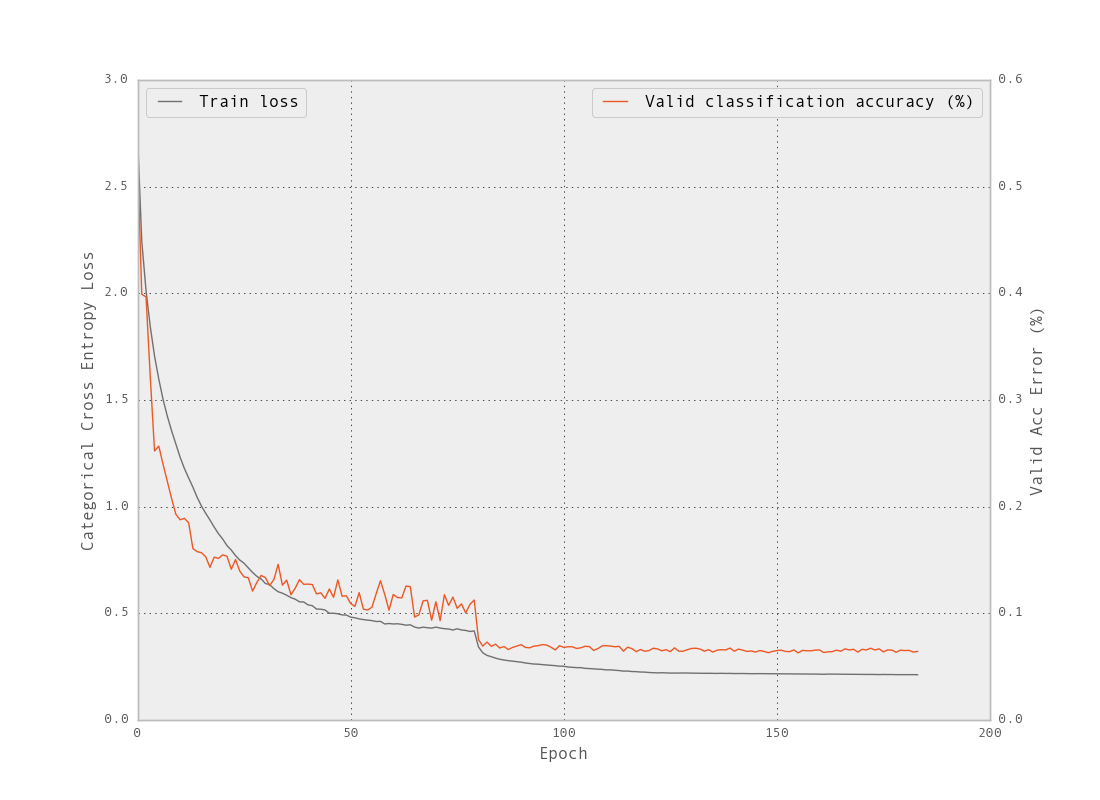
\includegraphics{images/preresnet_110_plot.png}
\caption{ResNet-110}
\end{figure}

\subsubsection{ResNet-164}\label{resnet-164}

\begin{figure}[htbp]
\centering
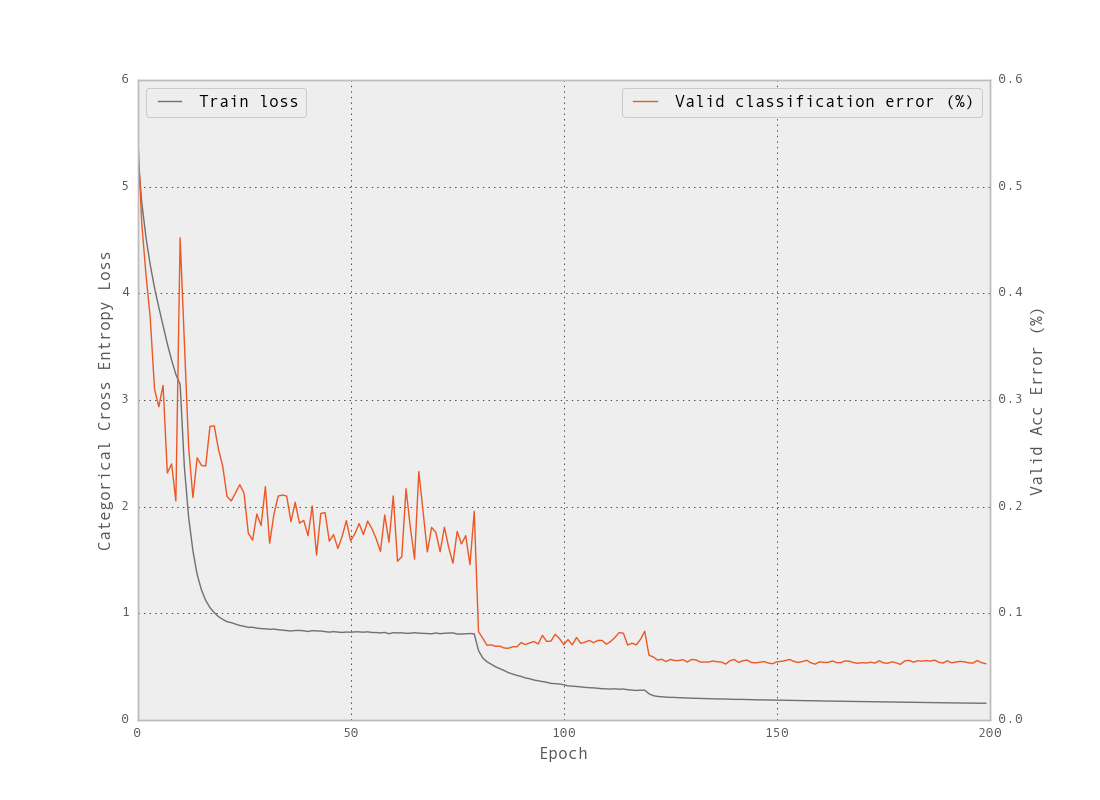
\includegraphics{images/preresnet_164_plot.png}
\caption{ResNet-164}
\end{figure}

\subsubsection{Wide-ResNet n=2 k=4}\label{wide-resnet-n2-k4}

\begin{figure}[htbp]
\centering
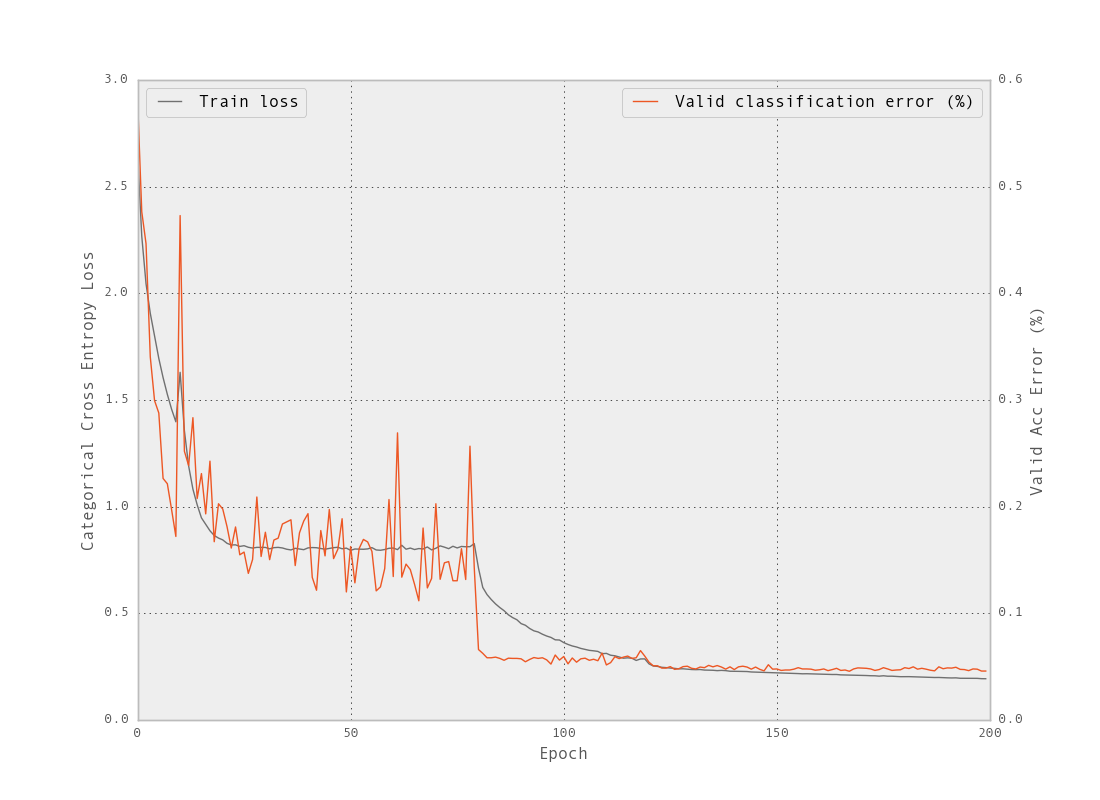
\includegraphics{images/wideresnet_n2_k4_plot.png}
\caption{Wide-ResNet}
\end{figure}

Finally, the speed of the networks may be interesting to some users.
Wide residual networks do seem to allow for more parameters with a
minimal cost in training time.

\begin{longtable}[c]{@{}ccc@{}}
\toprule
\textbf{ResNet Type} & \textbf{Params} &
\textbf{Sec/Epoch}\tabularnewline
\midrule
\endhead
ResNet-110 & 1.7M & 90\tabularnewline
ResNet-164 & 1.7M & 183\tabularnewline
WResNet-n2-k4 & 2.7M & 113\tabularnewline
\bottomrule
\end{longtable}

\section{Conclusion}\label{conclusion}

The results from the original two papers were reproduced within a small
margin which is to be expected given the stochastic properties of neural
networks. Additionally the results from the wide residual networks were
able to be reproduced even with slightly different preprocessing and
training parameters. This underscores the robust qualities and high
performance of these new neural network architectures.

\section{References}\label{references}

\begin{itemize}
\tightlist
\item
  {[}1{]} He, Kaiming, et al. ``Deep residual learning for image
  recognition.'' arXiv preprint arXiv:1512.03385 (2015).
  \href{https://arxiv.org/abs/1512.03385}{link}
\item
  {[}2{]} He, Kaiming, et al. ``Identity mappings in deep residual
  networks.'' arXiv preprint arXiv:1603.05027 (2016).
  \href{https://arxiv.org/abs/1603.05027}{link}
\item
  {[}3{]} Sergey Zagoruyko, Nikos Komodakis, ``Wide Residual Neural
  Networks.'' arXiv preprint arXiv:1605.07146 (2016).
  \href{https://arxiv.org/abs/1605.07146}{link}
\item
  {[}4{]} The Theano Development Team, et al. ``Theano: A Python
  framework for fast computation of mathematical expressions.'' arXiv
  preprint arXiv:1605.02688 (2016).
  \href{https://arxiv.org/abs/1605.02688}{link}
\item
  {[}5{]} Dieleman, Sander, et al. ``Lasagne: First Release.'' Zenodo:
  Geneva, Switzerland (2015).
  \href{http://lasagne.readthedocs.io/en/latest/index.html}{link}
\item
  {[}6{]} Collobert, Ronan, Koray Kavukcuoglu, and Clément Farabet.
  ``Torch7: A matlab-like environment for machine learning.'' BigLearn,
  NIPS Workshop. No. EPFL-CONF-192376. (2011).
  \href{http://cs.nyu.edu/~koray/files/2011_torch7_nipsw.pdf}{link}
\end{itemize}

{\sffamily \small
  \printbibliography
}
\end{document}
